\documentclass[a4paper]{article}

\usepackage[utf8]{inputenc}
\usepackage[portuguese]{babel}
\usepackage{a4wide}
\usepackage[pdftex]{hyperref}
\usepackage{graphicx}
\usepackage{wrapfig}
\usepackage{amsmath}
\usepackage{verbatim}
\usepackage{caption}
\usepackage{subcaption}
\usepackage{float}
\usepackage{blochsphere}



\begin{document}

\begin{titlepage}
\begin{center}



\includegraphics[width=0.4\textwidth]{logo.jpg}\\[0.5cm]

\vspace{10mm}

{\huge Universidade do Minho - Escola de Engenharia}\\[0.5cm]

{\large Relatório do trabalho prático de Computação Gráfica}\\[0.5cm]

\vspace{10mm} 

% Title
\rule{\linewidth}{0.5mm} \\[0.4cm]
{ \huge \bfseries Fase 1 – Primitivas Gráficas \\[0.4cm] }
\rule{\linewidth}{0.5mm} \\[1.5cm]

% Author and supervisor
\noindent
\begin{minipage}{0.4\textwidth}
  \begin{flushleft} \large
    \emph{Autores :}\\
    Daniel Maia \textsc{(A77531)}\\
    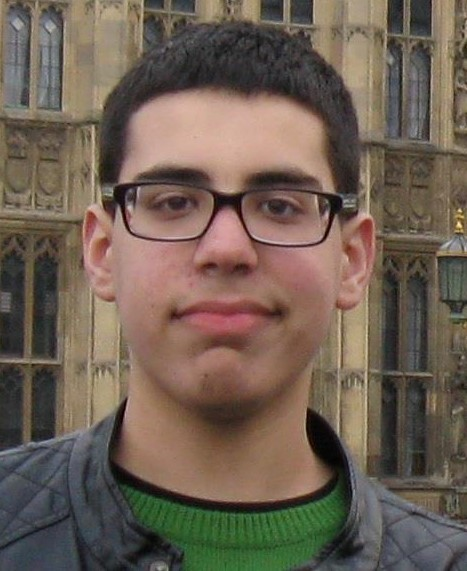
\includegraphics[width=1.5cm]{daniel.jpg}\break
    Diogo Silva\textsc{(A78034)}\\
    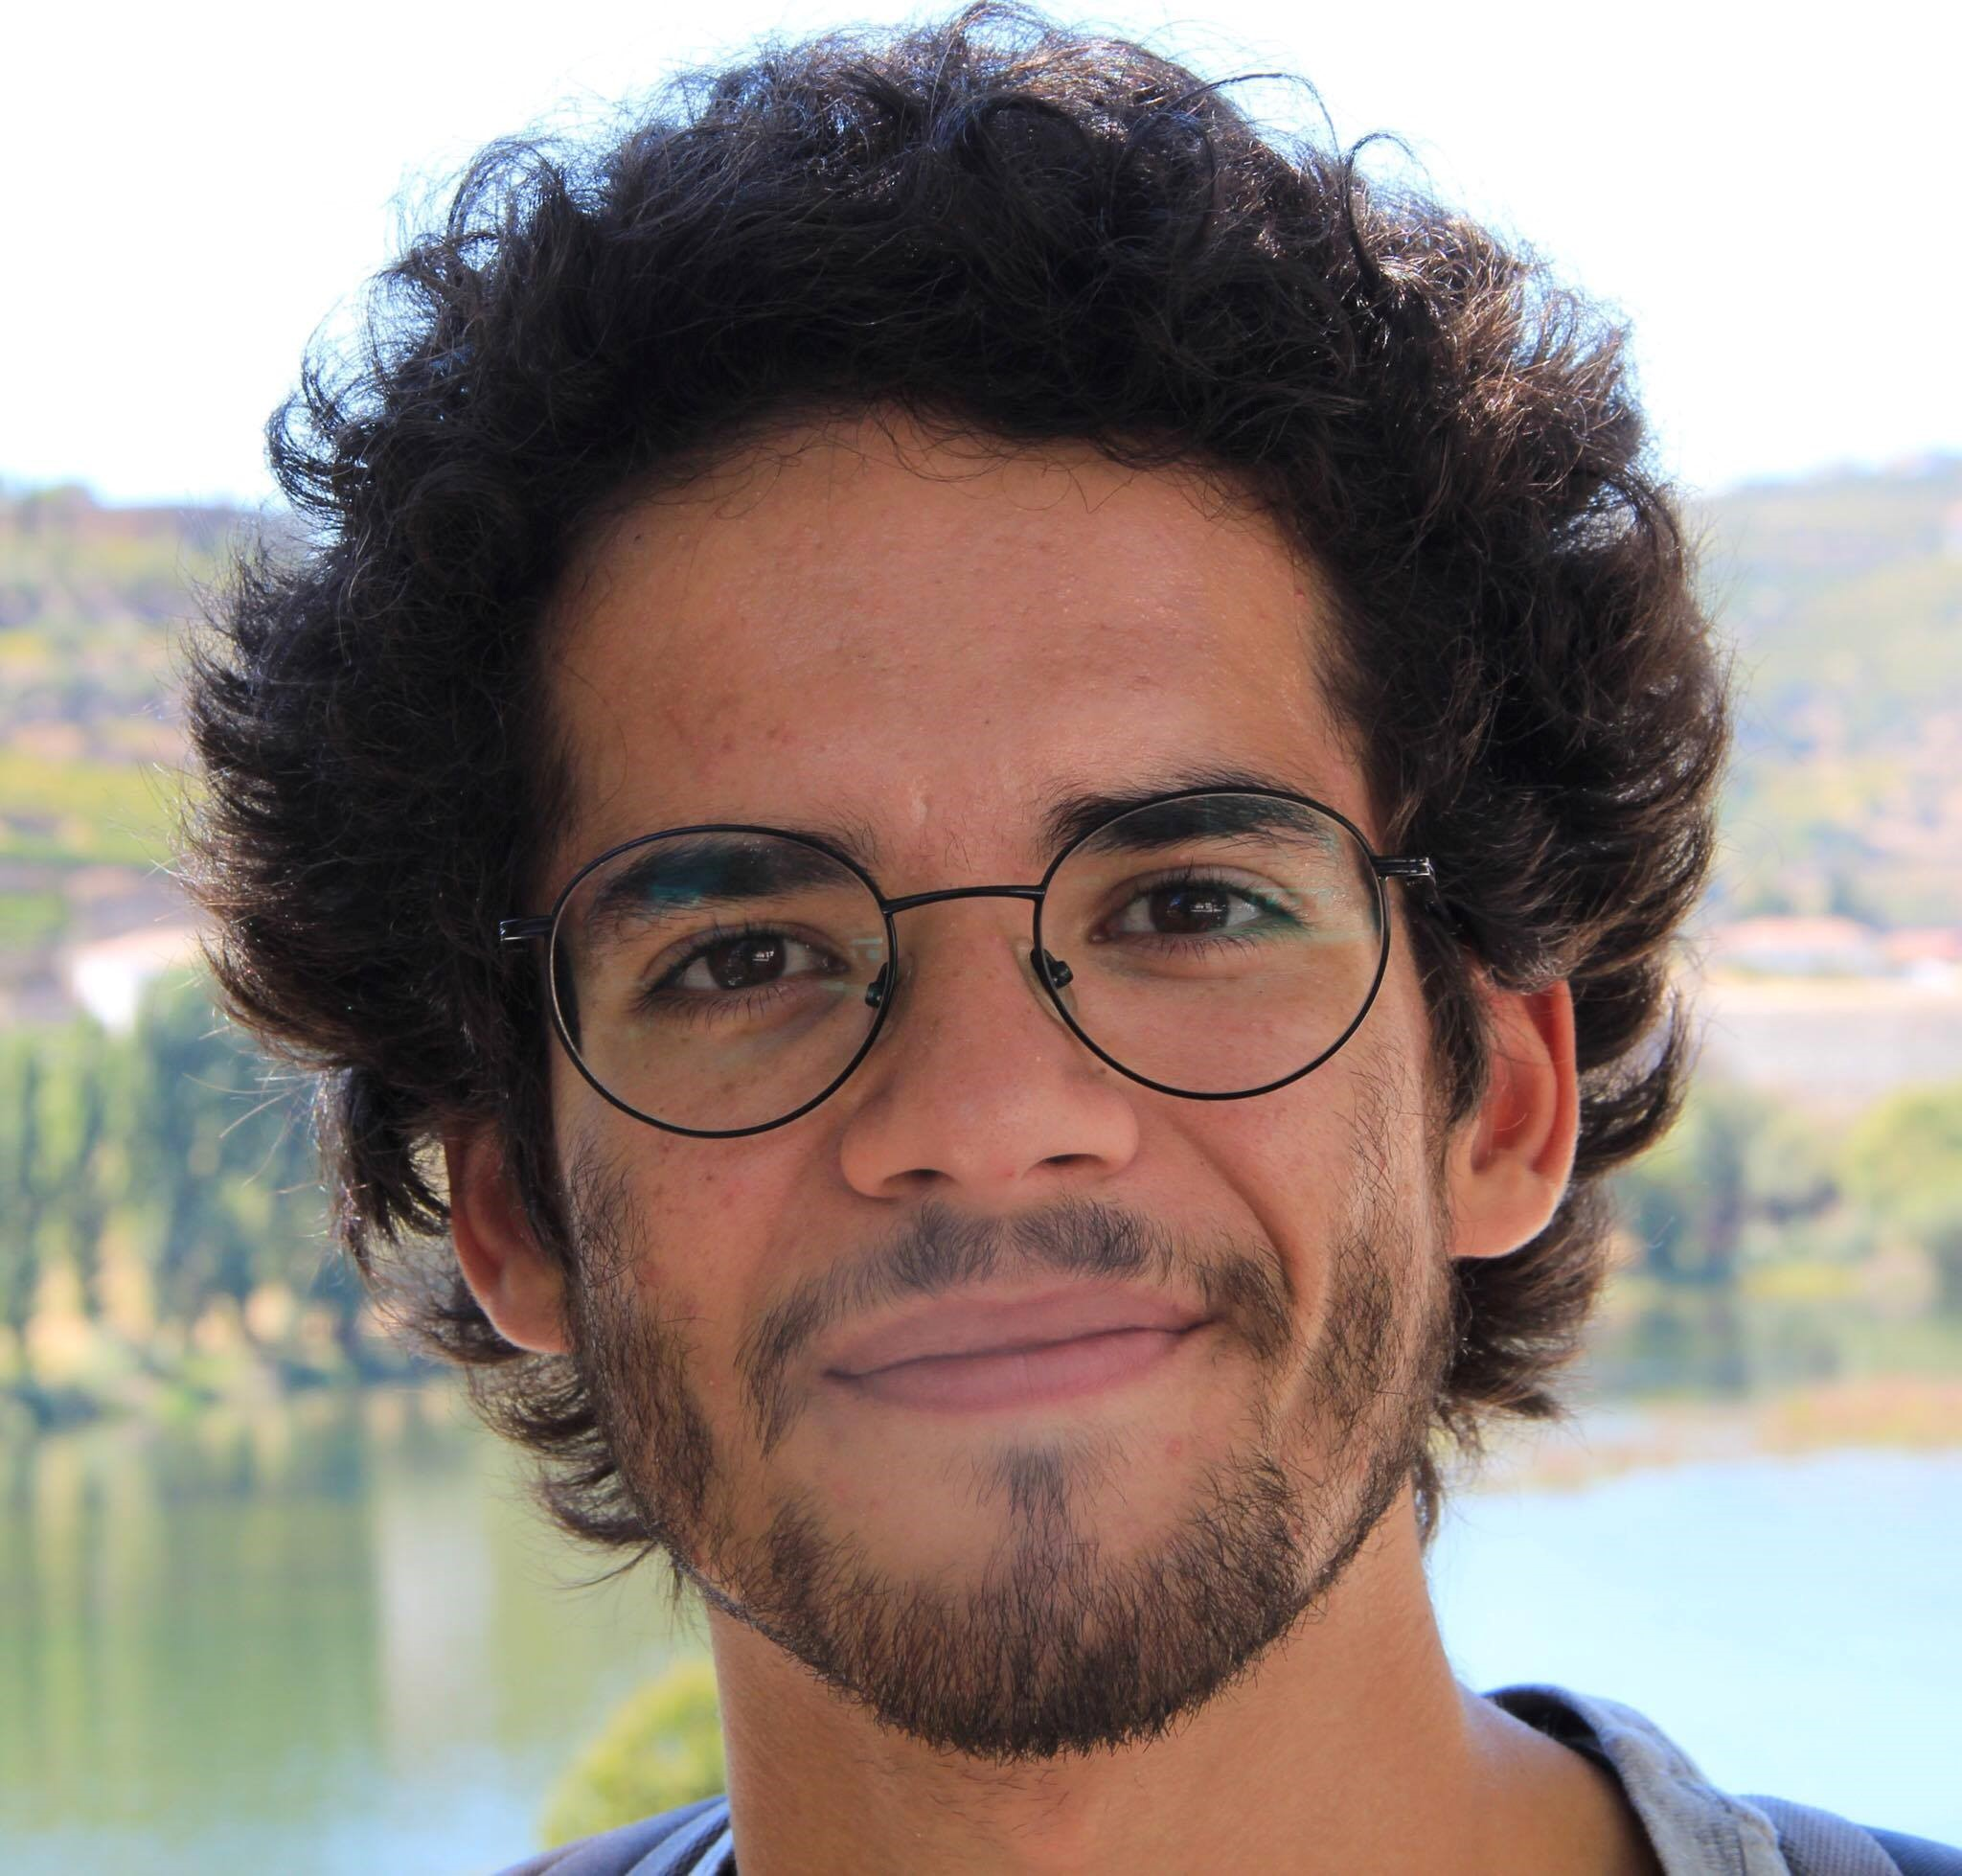
\includegraphics[width=1.5cm]{afonso.jpg}\break
    Marco Silva\textsc{(A79607)}\\
    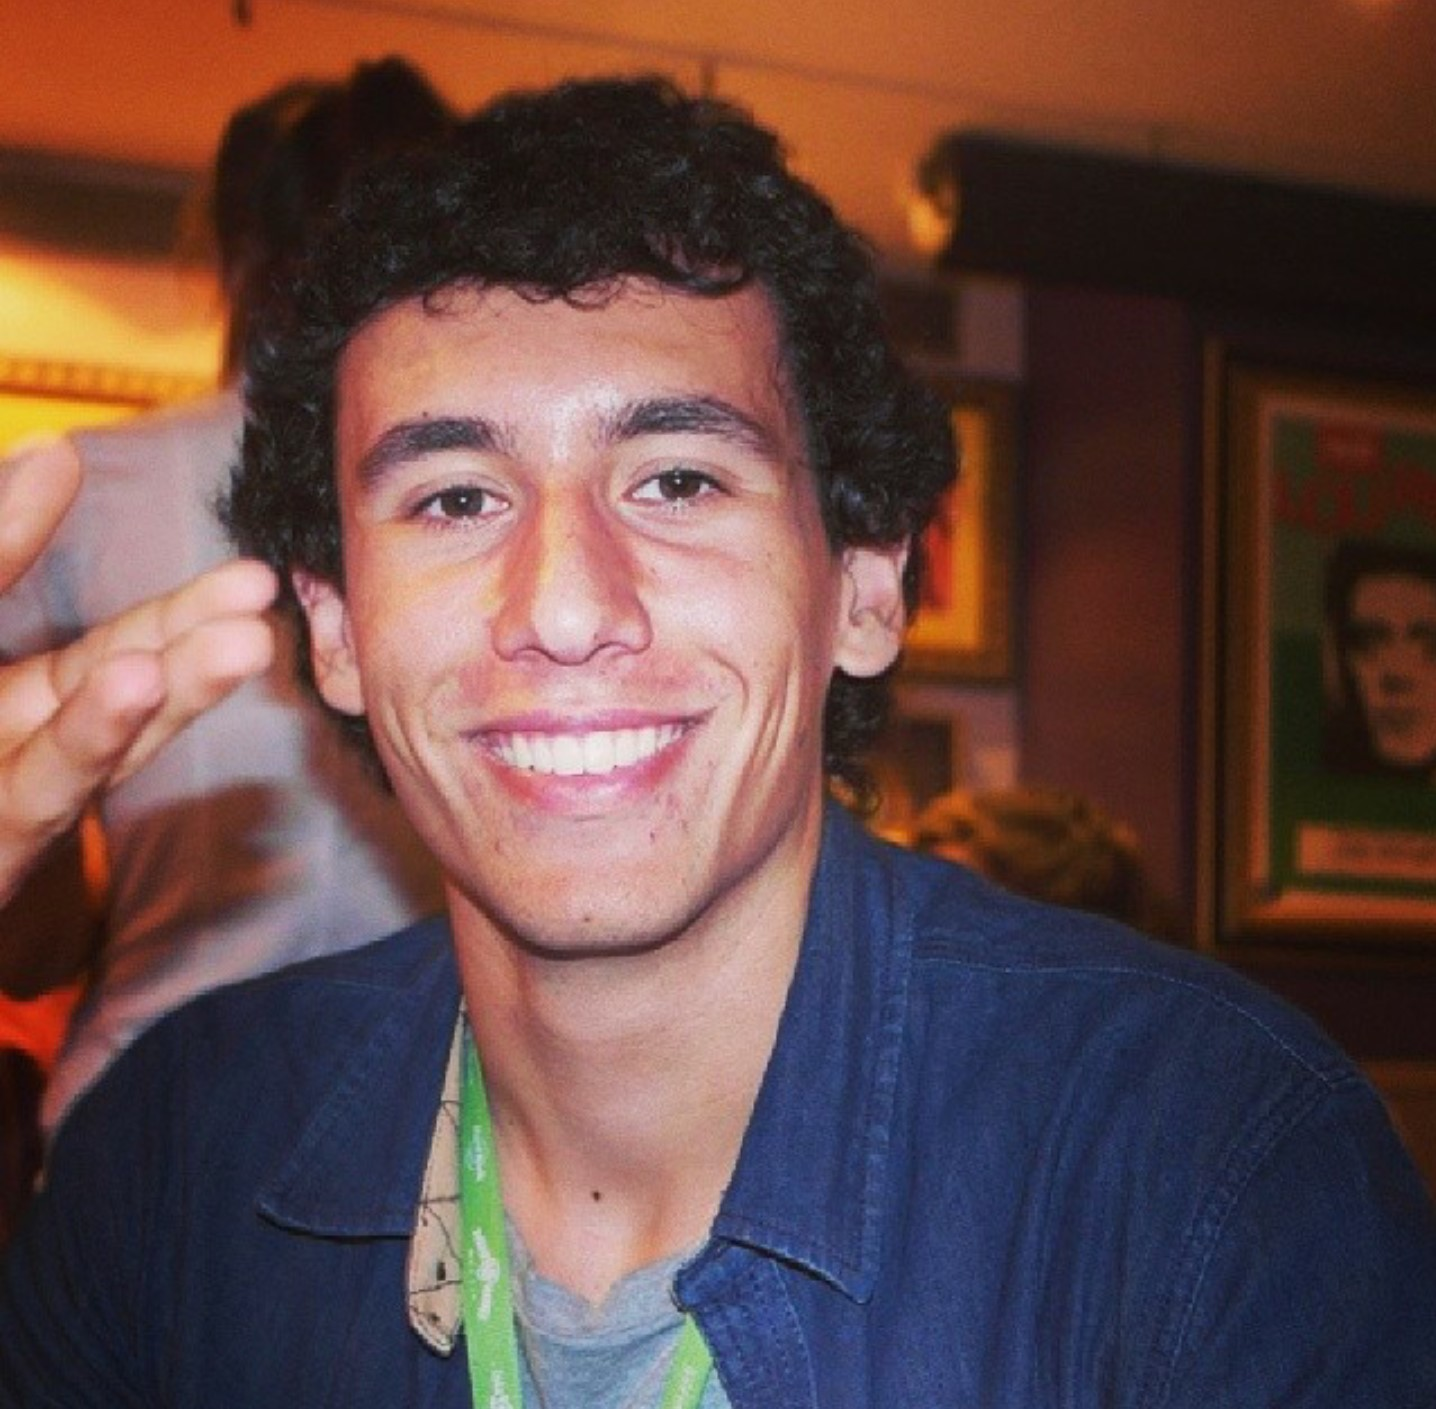
\includegraphics[width=1.5cm]{marco.jpg}\break
  \end{flushleft}
\end{minipage}%
\vfill


\begin{blochsphere}[radius=1.5 cm,tilt=15,rotation=-20,opacity=0]
    \drawBallGrid[style={opacity=0.1}]{30}{30}

    \drawGreatCircle[style={dashed}]{-60}{0}{0}
    \drawGreatCircle[style={dashed}]{60}{0}{0}

    \drawRotationLeft[scale=1.3,style={red}]{-60}{0}{0}{15}
    \drawRotationRight[scale=1.3,style={red}]{60}{0}{0}{15}

    \node at (-0.8,1.9) {\textcolor{red}{\tiny $J_{12}(t)$}};
    \node at (1.1,1.8) {\textcolor{red}{\tiny $J_{23}(t)$}};

    \labelLatLon{up}{90}{0};
    \labelLatLon{down}{-90}{90};
    \node[above] at (up) {{\tiny $\left|1\right>$ }};
    \node[below] at (down) {{\tiny $\left|0\right>$}};

    \labelLatLon[labelmark=false]{d}{15}{90};
    \node at (d) {\color{gray}\fontsize{0.15cm}{1em}\selectfont $60^\circ$};

    \labelLatLon[labelmark=false]{d2}{5}{78};
    \node at (d2) {\color{gray}\fontsize{0.15cm}{1em}\selectfont $60^\circ$};
\end{blochsphere}

% Bottom of the page
{\large Versão 1.0 \\ \today}

\end{center}
\end{titlepage}


\begin{abstract}

\hspace{3mm} 

\end{abstract}

\pagebreak
\tableofcontents

\pagebreak

% ===================================================
\section{Introdução}


% ===================================================
\section{Preliminares}


% ===================================================
\section{Descrição do Trabalho e Análise de Resultados}


% ===================================================
\section{Conclusões e Sugestões}


% ===================================================
\section{Referências}


% ===================================================
\section{Anexos}

\end{document}